\chapter[Hierarchical Selective Classification]{Hierarchical Selective Classification of European Land Use / Land Cover using pixel-based uncertainty}
\label{cha:chapter4}
\vspace*{\fill}
This chapter is based on:
\\
\\
% Full citation of the published (or submitted/in review) article
% This refers to the article key in the refs.bib file.
\fullcite{witjes2024hierarchical}
\newpage

\section*{Abstract}
HAS TO HAVE ALL SECTIONS

CAN BE SHORT AND UNCOOKED

SOME CLEAR RESULTS
\newpage

\section{Introduction}
Land cover is important. 

\subsection{Land cover mapping}

    \subsection{Where do you get data?}
    
        It is important to have independent training and validation samples. The best open validation samples for Europe are the LUCAS points \citep{dandrimont2021lucas,dandrimont2020harmonised} because of their sound sampling design, large legend, and covering multiple years \citep{venter2022global}
        
        Corine is super cool and can be harvested for training data\citep{witjes2022spatiotemporal,witjes2024iterative}
        but doesn't have all classes for LUCAS validation \citep{dandrimont2021lucas} if you want to go beyond high level classes or throw a lot away \citep{pflugmacher2019mapping}.
        Eurocrops is super cool and provides a lot of classes missing in CORINE \citep{schneider2023eurocrops}
        OpenStreetMap is super cool and can be used to supplement training datasets with additional classes [SOURCE NEEDED] and can also be used to filter spurious labels extracted from CORINE \citep{witjes2022spatiotemporal}

    \subsection{Detail and accuracy}
        
        Mapping many classes is more difficult:
        \begin{enumerate}
        \item Collecting training and validation samples
        \item Model training (more confusion)
        \item Map interpretability (harder to read)
        \end{enumerate}
        It is not often done at high spatial resolution.

    \subsection{Prediction uncertainty}
        Prediction uncertainty = the chance that a specific prediction is correct.
        You can use heuristics but they don't give a statistical guarantee. Examples are the predicted probabilities, especially if they are well-calibrated \citep{niculescu2005predicting}, the margin of victory (the difference between the probabilities of the highest and second highest class) \citep{calderon-loor2021high}, and model variance from ensembles of classifiers \citep{witjes2022spatiotemporal}. \citet{witjes2024iterative} found indications of a relationship between a prediction's certainty and the iteration at which it is classified by IMP.

    \subsection{Selective classification}

    \subsection{hierarchical classification}
        you can first predict level 1 and then level 2, but then there's error propopagation

    \subsection{Research gaps}
        It is likely that prediction uncertainty will be higher when there are more classes in a legend, especially when they are spectrally similar, such as different cereal types. This introduces errors in the map that could be avoided by having a simpler legend, but this sacrifices thematic depth for accuracy There is a need for maps that are more detailed than the typical 'artificial, forest, cropland, grasland, water' type classes, so navigating the trade-off between accuracy and detail must be done.

    \subsection{This paper}
        In this paper, we demonstrate an improved version of the framework proposed by \citep{witjes2022spatiotemporal} to extract training data from multiple open land cover polygon datasets (Eurocrops, OpenStreetmap, and Corine Land Cover) from several years across Europe. 
        
        We train a land cover classification model and predict probabilities for 53 LUCAS land cover classes.
        
        We create hard-class maps using maximum probability assignment and Iterative Mapping of Probabilities (IMP) \citep{witjes2024iterative} for each level in the hierarchical legend, and then aggregate uncertain predictions to a higher level in the legend to minimize error. We compare three different uncertainty metrics: The highest predicted probability and margin of victory (difference between the highest and second highest), and the iteration at which a pixel was classified during IMP.
        
        Each metric is used to generate hard class maps where uncertain predictions are aggregated to more general classes (e.g. \textit{Rice} and \textit{Wheat} to \textit{Cereals}, and \textit{Cereals} and \textit{Root crops} to \textit{Cropland}). We validate the resulting hard class maps with LUCAS land cover observations, and assess how well each metric can be used to navigate the trade-off between accuracy and detail.

\section{Methods}

\begin{figure}[H]
    \centering
    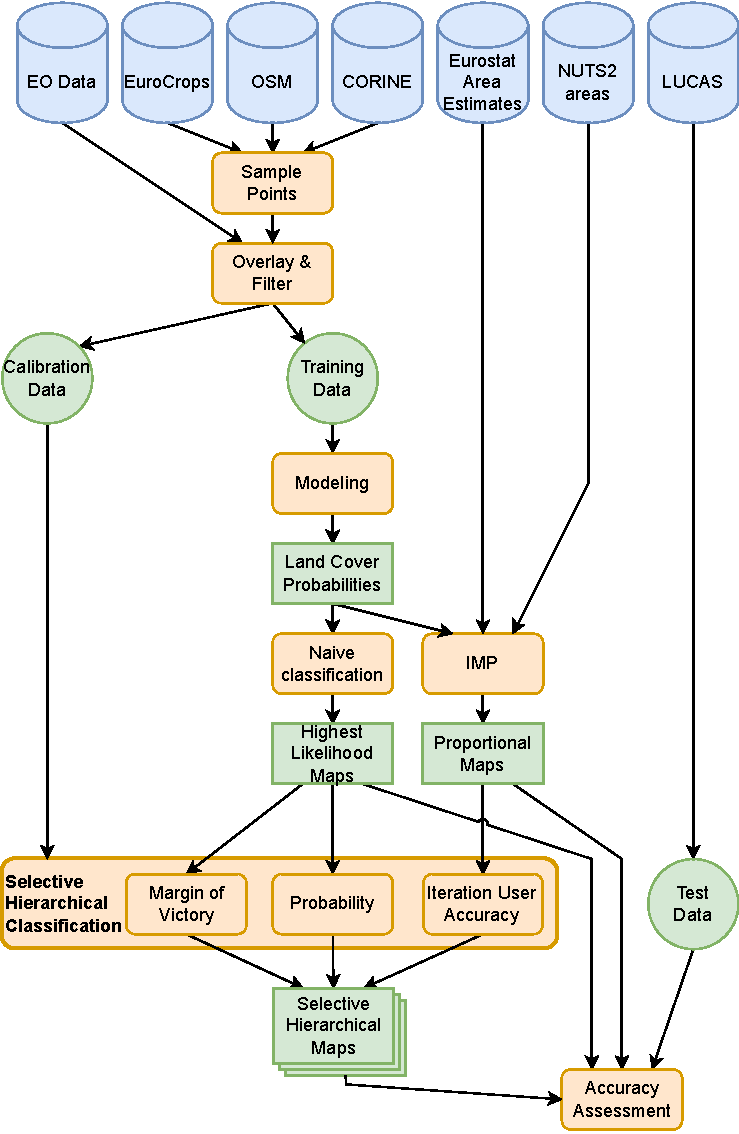
\includegraphics[width=\textwidth]{figs_05/fig_methodology.pdf}
    \caption{Caption}
    \label{fig:05_methodology}
\end{figure}

\subsection{Selection of study area}

We obtained Nomenclature of Territorial Units for Statistics (NUTS) administrative boundaries from EuroStat. %https://ec.europa.eu/eurostat/web/gisco/geodata/reference-data/administrative-units-statistical-units/nuts
We matched level 2 NUTS areas to the earliest LUCAS survey since each update (See Table~\ref{tab:05_NUTS_LUCAS}). 

We selected all NUTS2 areas:
1. For which LUCAS land cover area estimates were available;
2. For which more than 500 LUCAS points were available;
2. Whose area was below the largest 1\% surface area among NUTS2 areas (to maintain computational feasibility)

We randomly selected up to four NUTS2 area/year combinations each country.

\begin{table}[H]
    \centering
    \begin{tabular}{c|c}
         NUTS update year &  LUCAS survey year\\
         2006 & 2006 \\
         2010 & 2012 \\
         2013 & 2015 \\
         2016 & 2018 \\
    \end{tabular}
    \caption{Caption}
    \label{tab:05_NUTS_LUCAS}
\end{table}

\subsection{Legend harmonization}
% https://docs.google.com/spreadsheets/d/1UJrbdGJgrXlW_WnSoDVIhf68dz8XoiWrZW6WVeR5lPw/edit#gid=1654270911
For some classes, either no area estimates or no training data was found. This required us to merge some classes, and aggregate others to a higher level in the hierarchical legend. Table \ref{tab:05_legend_harmonization} shows which LUCAS classes were aggregated and merged, and for what reason.

% Please add the following required packages to your document preamble:
% \usepackage{multirow}
\begin{table}[]
\label{tab:05_legend_harmonization}
% https://docs.google.com/spreadsheets/d/1UJrbdGJgrXlW_WnSoDVIhf68dz8XoiWrZW6WVeR5lPw/edit#gid=213241018
\begin{tabular}{l{2cm}lll}
LUCAS land cover class                        & Training data source    & Used land cover class                                 & Reason for aggregation/omission                           \\
A11: Buildings with one to three floors       & \multirow{2}{*}{corine} & \multirow{2}{*}{A10: Roofed built-up areas}           & No training data                                          \\
A12: Buildings with more than three floors    &                         &                                                       & No training data                                          \\
\multirow{2}{*}{A13: Greenhouses}             & openstreetmap           & \multirow{2}{*}{A13: Greenhouses}                     &                                                           \\
                                              & eurocrops               &                                                       &                                                           \\
A21: Non built-up area features               & \multirow{2}{*}{corine} & \multirow{2}{*}{A20: Artificial non-built up areas}   & No training data                                          \\
A22: Non built-up linear features             &                         &                                                       & No training data                                          \\
B11: Common wheat                             & eurocrops               & B11: Common wheat                                     &                                                           \\
B12: Durum wheat                              & eurocrops               & B12: Durum wheat                                      &                                                           \\
B13: Barley                                   & eurocrops               & B13: Barley                                           &                                                           \\
B14: Rye                                      & eurocrops               & B14: Rye                                              &                                                           \\
B15: Oats                                     & eurocrops               & B15: Oats                                             &                                                           \\
B16: Maize                                    & eurocrops               & B16: Maize                                            &                                                           \\
B17: Rice                                     & corine                  & B17: Rice                                             &                                                           \\
B17: Rice                                     & eurocrops               & B17: Rice                                             &                                                           \\
B18: Triticale                                & eurocrops               & B18: Triticale                                        &                                                           \\
B19: Other cereals                            & eurocrops               & \multirow{2}{*}{B19: Other cereals}                   &                                                           \\
B54: Mixed cereals for fodder                 &                         &                                                       & No training data                                          \\
B21: Potatoes                                 & eurocrops               & B21: Potatoes                                         &                                                           \\
B22: Sugar beet                               & eurocrops               & B22: Sugar beet                                       &                                                           \\
B23: Other root crops                         & eurocrops               & B23: Other root crops                                 &                                                           \\
B31: Sunflower                                & eurocrops               & B31: Sunflower                                        &                                                           \\
B32: Rape and turnip rape                     & eurocrops               & B32: Rape and turnip rape                             &                                                           \\
B33: Soya                                     & eurocrops               & B33: Soya                                             &                                                           \\
B34: Cotton                                   & eurocrops               & \multirow{2}{*}{B35: Other fibre and olaginous crops} & No training data in eurocrops, despite presence in legend \\
B35: Other fibre and olaginous crops          & eurocrops               &                                                       &                                                           \\
B36: Tobacco                                  & eurocrops               & B36: Tobacco                                          &                                                           \\
B37: Other non-permanent industrial crops     & eurocrops               & B37: Other non-permanent industrial crops             &                                                           \\
B41: Dry pulses                               & eurocrops               & B41: Dry pulses                                       &                                                           \\
B42: Tomatoes                                 & eurocrops               & B42: Tomatoes                                         &                                                           \\
B43: Other fresh vegetables                   & eurocrops               & B43: Other fresh vegetables                           &                                                           \\
B44: Floriculture and ornamental plants       & eurocrops               & B44: Floriculture and ornamental plants               &                                                           \\
B45: Strawberries                             & eurocrops               & B45: Strawberries                                     &                                                           \\
B51: Clovers                                  & eurocrops               & B51: Clovers                                          &                                                           \\
B52: Lucerne                                  & eurocrops               & B52: Lucerne                                          &                                                           \\
B53: Other leguminous and mixtures for fodder & eurocrops               & B53: Other leguminous and mixtures for fodder         &                                                           \\
B55: Temporary grasslands                     & eurocrops               & B55: Temporary grasslands                             &                                                           \\
B71: Apple fruit                              & eurocrops               & B71: Apple fruit                                      &                                                           \\
B72: Pear fruit                               & eurocrops               & B72: Pear fruit                                       &                                                           \\
B73: Cherry fruit                             & eurocrops               & B73: Cherry fruit                                     &                                                           \\
B74: Nuts trees                               & eurocrops               & B74: Nuts trees                                       &                                                           \\
B75: Other fruit trees and berries            & eurocrops               & B75: Other fruit trees and berries                    &                                                           \\
B76: Oranges                                  &                         & \multirow{2}{*}{B77: Other citrus fruit}              & No training data                                          \\
B77: Other citrus fruit                       & eurocrops               &                                                       &                                                           \\
\multirow{2}{*}{B81: Olive groves}            & corine                  & \multirow{2}{*}{B81: Olive groves}                    &                                                           \\
                                              & eurocrops               &                                                       &                                                           \\
\multirow{2}{*}{B82: Vineyards}               & corine                  & \multirow{2}{*}{B82: Vineyards}                       &                                                           \\
                                              & eurocrops               &                                                       &                                                           \\
B83: Nurseries                                & eurocrops               & B83: Nurseries                                        &                                                           \\
B84: Permanent industrial crops               & eurocrops               & B84: Permanent industrial crops                       &                                                           \\
C10: Broadleaved woodland                     & corine                  & C10: Broadleaved woodland                             &                                                           \\
C21: Spruce dominated coniferous woodland     & \multirow{3}{*}{corine} & \multirow{3}{*}{C20: Coniferous woodland}             & No area estimates                                         \\
C22: Pine dominated coniferous woodland       &                         &                                                       & No area estimates                                         \\
C23: Other coniferous woodland                &                         &                                                       & No area estimates                                         \\
C31: Spruce dominated mixed woodland          & \multirow{3}{*}{corine} & \multirow{3}{*}{C30: Mixed woodland}                  & No area estimates                                         \\
C32: Pine dominated mixed woodland            &                         &                                                       & No area estimates                                         \\
C33: Other mixed woodland                     &                         &                                                       & No area estimates                                         \\
D10: Shrubland with sparse tree cover         & corine                  & D10: Shrubland with sparse tree cover                 &                                                           \\
D20: Shrubland without tree cover             & corine                  & D20: Shrubland without tree cover                     &                                                           \\
E10: Grassland with sparse tree/shrub cover   &                         & \multirow{4}{*}{E00: Grassland}                       & No training data                                          \\
E20: Grassland without tree/shrub cover       & eurocrops               &                                                       & No area estimates                                         \\
E20: Grassland without tree/shrub cover       & corine                  &                                                       & No area estimates                                         \\
E30: Spontaneously re-vegetated surfaces      &                         &                                                       & no training data                                          \\
F10: Rocks and stones                         & \multirow{3}{*}{corine} & \multirow{3}{*}{F00: Bare land and lichens/moss}      & No area estimates                                         \\
F20: Sand                                     &                         &                                                       & No area estimates                                         \\
F40: Other bare soil                          &                         &                                                       & No area estimates                                         \\
G11: Inland fresh water bodies                & \multirow{8}{*}{corine} & \multirow{8}{*}{G00: Water areas}                     & No area estimates                                         \\
G12: Inland salty water bodies                &                         &                                                       & No area estimates                                         \\
G21: Inland fresh running water               &                         &                                                       & No area estimates                                         \\
G22: Inland salty running water               &                         &                                                       & No area estimates                                         \\
G30: Transitional water bodies                &                         &                                                       & No area estimates                                         \\
G30: Transitional water bodies                &                         &                                                       & No area estimates                                         \\
G40: Sea and ocean                            &                         &                                                       & No area estimates                                         \\
G50: Glaciers, permanent snow                 &                         &                                                       & No area estimates                                         \\
H11: Inland marshes                           & \multirow{5}{*}{corine} & H11: Inland marshes                                   &                                                           \\
H12: Peatbogs                                 &                         & H12: Peatbogs                                         &                                                           \\
H21: Salt marshes                             &                         & H21: Salt marshes                                     &                                                           \\
H22: Salines and other chemical deposits      &                         & H22: Salines and other chemical deposits              &                                                           \\
H23: Intertidal flats                         &                         & H23: Intertidal flats                                 &                                                          
\end{tabular}
\end{table}

\subsection{Training and Calibration Samples}
We extracted polygons from CORINE, EuroCrops and OpenStreetmap. Table~\ref{tab:05_sources} shows the training data source per LUCAS class.

We randomly sampled points from polygons. One point minimum, one extra point per X square meters of polygon surface, to a maximum of X points per polygon.

We filtered the samples with Copernicus HRL layers and OpenStreetmap building and roads data. 

We split the samples in training and calibrations samples with a 0.75/0.25 split.



\subsection{Land Cover Classification}
We trained a LightGBM gradient boosting model \citep{ke2017lightgbm} on the training samples.
We predicted land cover probabilities on calibration points for all 53 LUCAS land cover classes and derived hard class maps using maximum probability assignment. For each calibration point, we stored the probability of the assigned class and the margin of victory.
We then applied the IMP algorithm on the calibration points, using the class distribution of the calibration points as a proxy of the area estimate.

% this should be on the calibration points from each NUTS2 area separately, using that area's area estimate.




\section{Results}
    \subsection{Training data}

        We sampled ~41 million points from the CORINE, EuroCrops and OpenStreetmap polygons. The filtering procedure removed ~25\% of samples, resulting in a dataset of 32 million samples, which was split into 24 million training samples and 8 million calibration samples.
    
\subsection{Validation data}

    Sampling one combination of a NUTS2 area and LUCAS survey year per country yielded 25 regions. Iteratively adding more area/year combinations to guarantee at least 30 LUCAS points per class in the validation dataset resulted in 17 more, with 9 of them being added to guarantee coverage of \textit{Intertidal Flats}, 3 for \textit{Strawberries}, and 3 for \textit{Tobacco}. This resulted in a total of 52 areas with at least 300 LUCAS observations, containing a total of 66994 observations. Figure~\ref{fig:05_lucas_aoi} shows all areas that were selected.
    
    \begin{figure}[h]
        \centering
        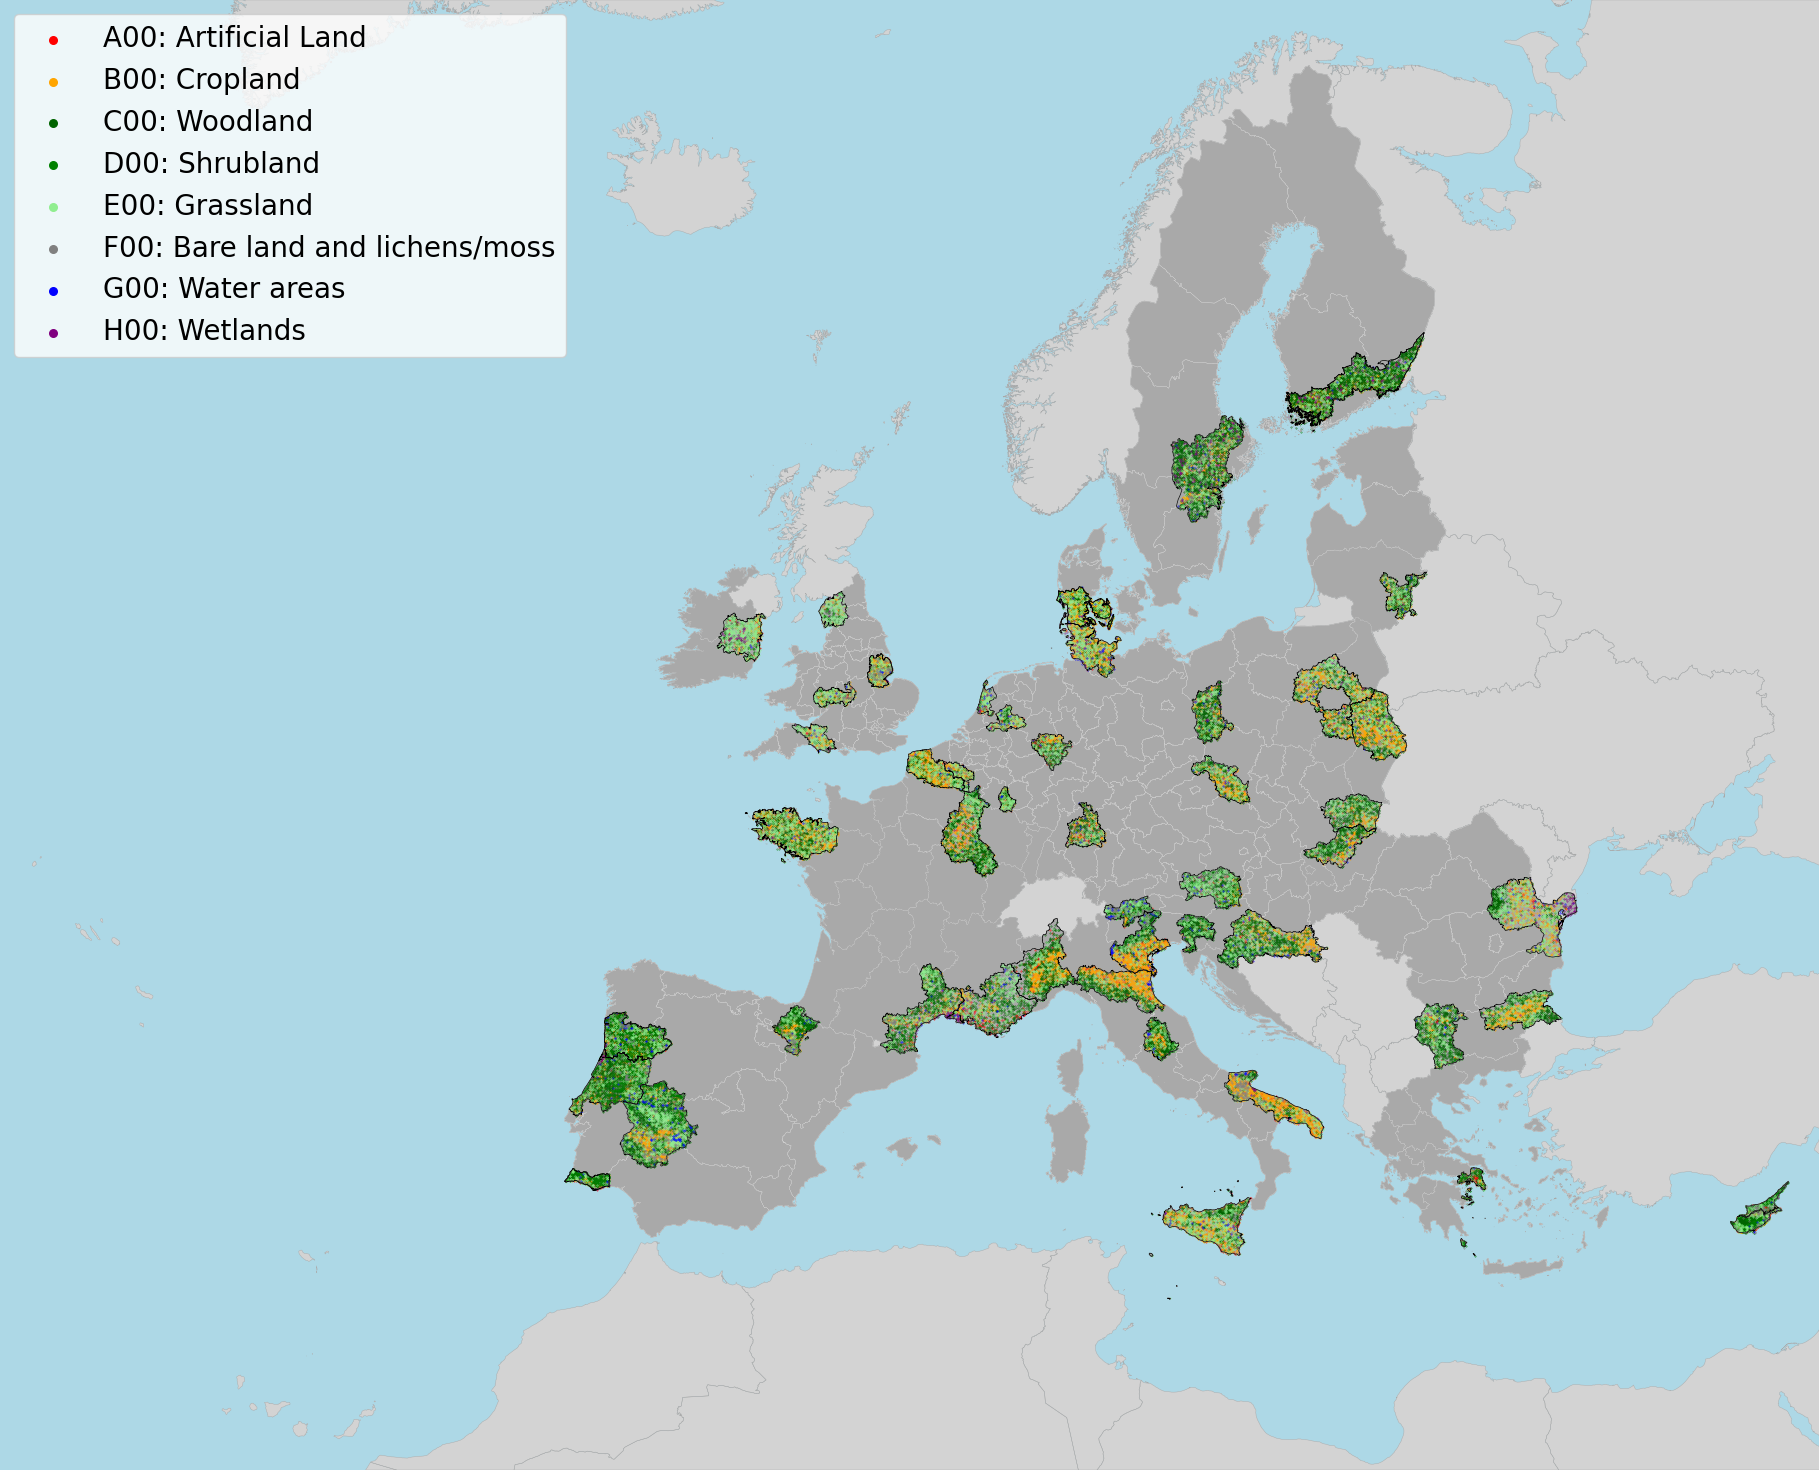
\includegraphics[width=\textwidth]{figs_05/fig_lucas_aoi.png}
        \caption{LUCAS points in sampled NUTS2 areas, used for validation of all land cover maps}
        \label{fig:05_lucas_aoi}
    \end{figure}
    
    \begin{figure}[h]
        \centering
        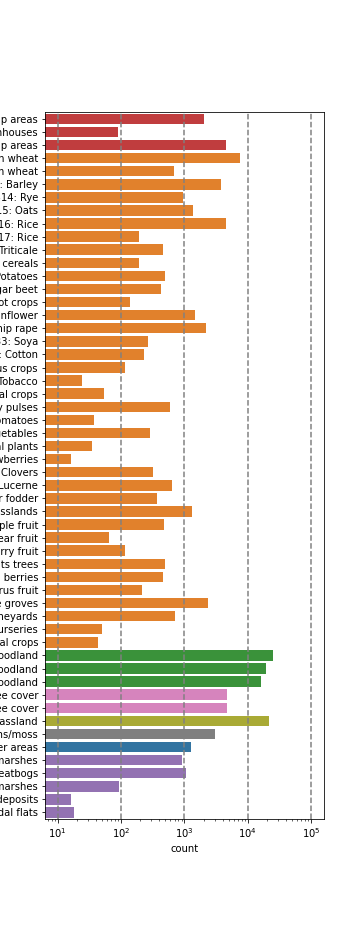
\includegraphics[width=\textwidth]{figs_05/fig_lucas_aoi_counts.png}
        \caption{Number of LUCAS points per LUCAS class used to validate the land cover maps, colored based on their level 1 class.}
        \label{fig:05_lucas_aoi_counts}
    \end{figure}

\subsection{Land Cover Modeling}

    The predicted probabilities on the calibration points were classified with both MPA and IMP on calibration points to assess their relative accuracy. Table \ref{tab:05_calibration_accuracy} shows that MPA produced the highest weighted precision at each level of the legend, while IMP produced the highest weighted F1-score by harmonizing precision and recall. The hierarchical confusion matrix in Figure~\ref{fig:05_confusion_matrix} shows that many crop types were frequently misclassified as \textit{Common Wheat}, \textit{Barley}, and \textit{Maize} within the textit{Cropland} level 1 class, while many cereal and fruit crops were frequently confused with \textit{Grassland}. 'Orchard' classes such as \textit{Apple fruit} and \textit{Pear fruit} orchards were also frequently confused with forest classes. The large non-hierarchical classes, Grassland, Bare Land, and Water, were among the most accurately classified, especially at level 3.
    
    \begin{table}[]
    \begin{tabular}{lrrrr}
    \textbf{Method} & \multicolumn{1}{l}{\textbf{Level}} & \multicolumn{1}{l}{\textbf{Precision}} & \multicolumn{1}{l}{\textbf{Recall}} & \multicolumn{1}{l}{\textbf{F1}} \\
    MPA & 1 & \textbf{0.76} & 0.70 & 0.69 \\
    MPA & 2 & 0.60 & 0.49 & 0.51 \\
    MPA & 3 & 0.59 & 0.45 & 0.48 \\
    IMP & 1 & 0.74 & \textbf{0.74} & \textbf{0.74} \\
    IMP & 2 & 0.57 & 0.57 & 0.57 \\
    IMP & 3 & 0.55 & 0.55 & 0.55
    \end{tabular}
    \caption{Weighted precision, recall and F1-score on calibration points at three levels in the LUCAS land cover hierarchy (8, 19, and 53 classes) by maximum probability assignment and iterative mapping of probabilities}
    \label{tab:05_calibration_accuracy}
    \end{table}

    \begin{table}[]
    \begin{tabular}{lrrrr}
    \textbf{Method} & \multicolumn{1}{l}{\textbf{Level}} & \multicolumn{1}{l}{\textbf{Precision}} & \multicolumn{1}{l}{\textbf{Recall}} & \multicolumn{1}{l}{\textbf{F1}} \\
    MPA & 1 & \textbf{0.66} & 0.57 & 0.58 \\
    MPA & 2 & 0.51 & 0.34 & 0.37 \\
    MPA & 3 & 0.47 & 0.29 & 0.33 \\
    IMP & 1 & 0.61 & \textbf{0.61} & \textbf{0.61} \\
    IMP & 2 & 0.43 & 0.43 & 0.43 \\
    IMP & 3 & 0.39 & 0.39 & 0.39
    \end{tabular}
    \caption{Weighted precision, recall and F1-score on LUCAS points at three levels in the LUCAS land cover hierarchy (8, 19, and 53 classes) by maximum probability assignment and iterative mapping of probabilities}
    \label{tab:05_calibration_accuracy}
    \end{table}

    \begin{figure}
        \centering
        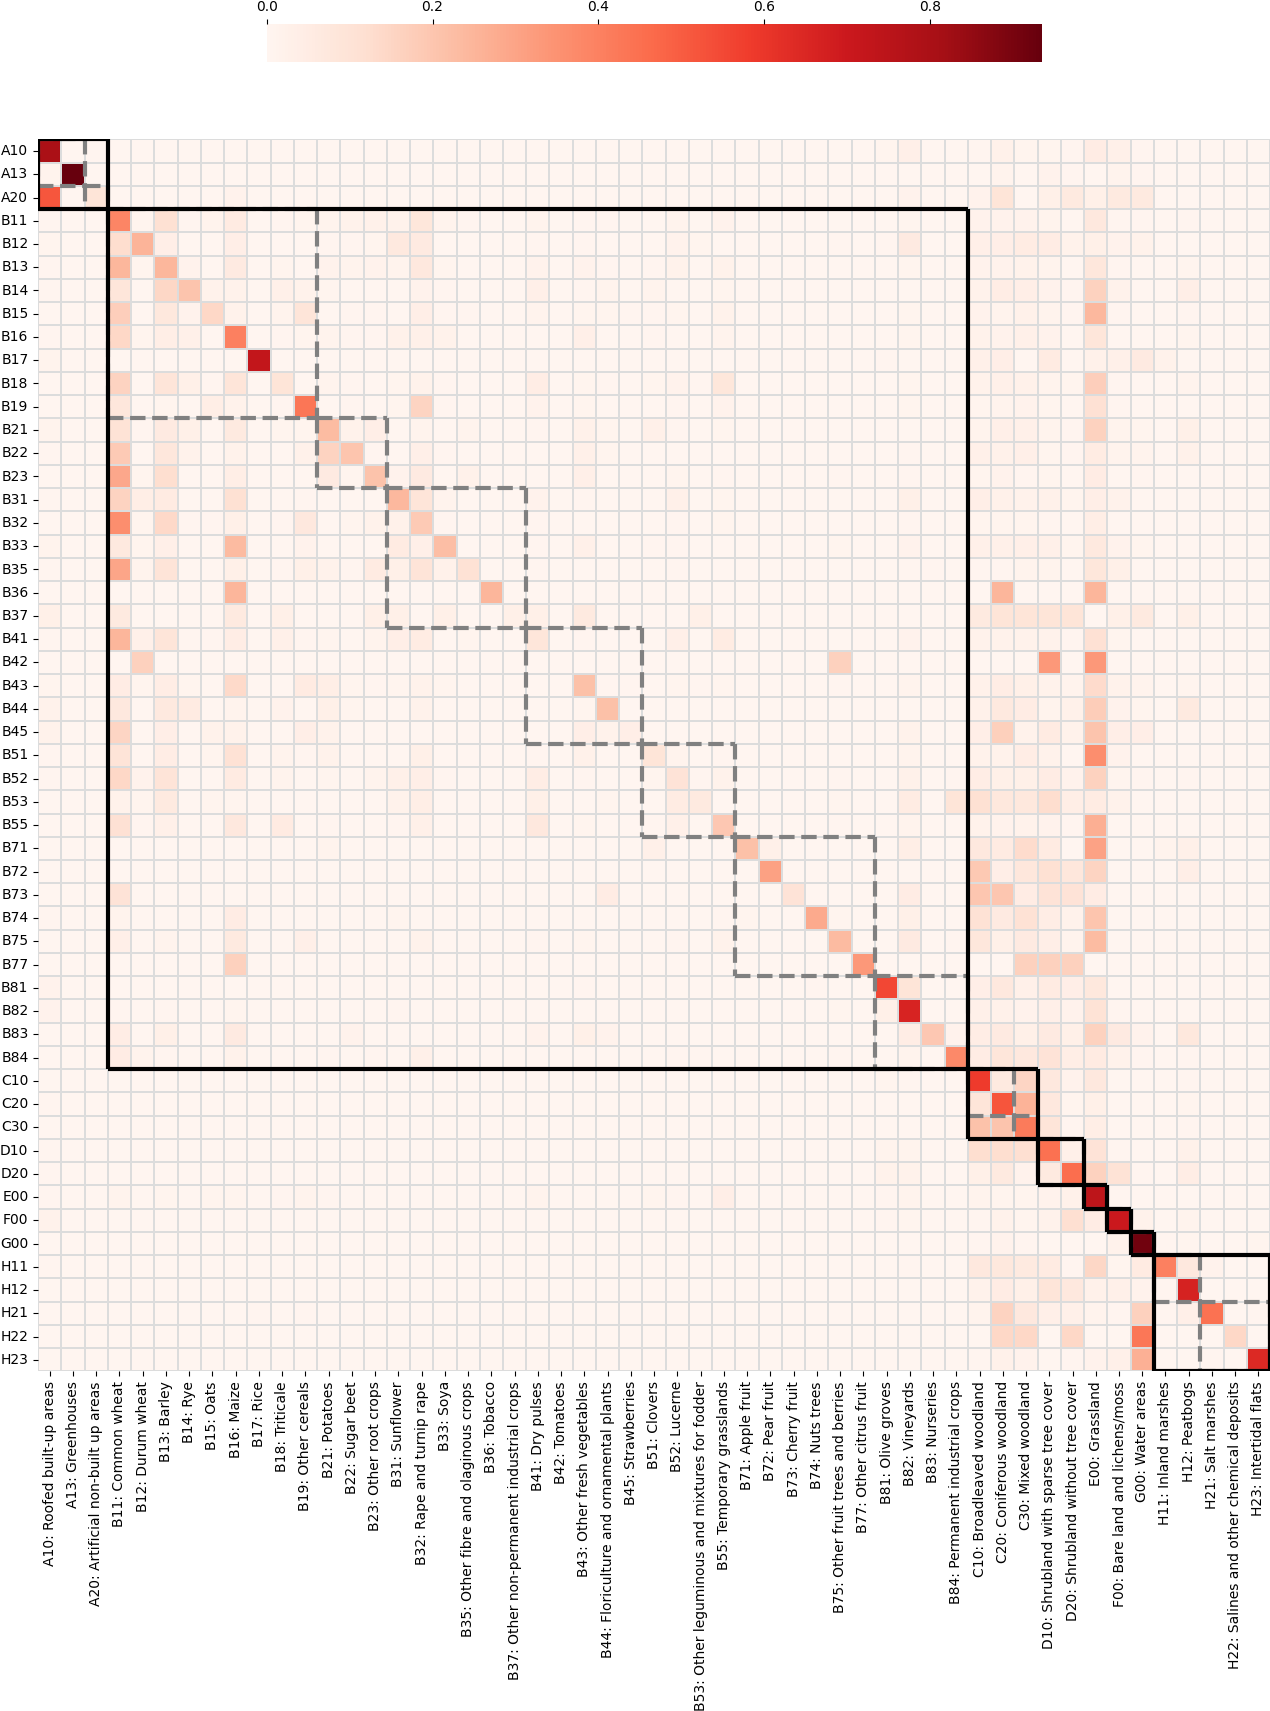
\includegraphics[width=\textwidth]{figs_05/fig_hierarchical_confusion_matrix_calib.png}
        \caption{Confusion matrix of the calibration points classified by IMP, normalized based on true class quantities. Red squares mean that the true class (x-axis) was often incorrectly predicted as the predicted class (y-axis)The grey dashed lines indicate which classes belong to the same level 2 class in the hierarchical legend. The black lines indicate level 1 class membership.}
        \label{fig:05_confusion_matrix}
    \end{figure}

    \begin{figure}
        \centering
        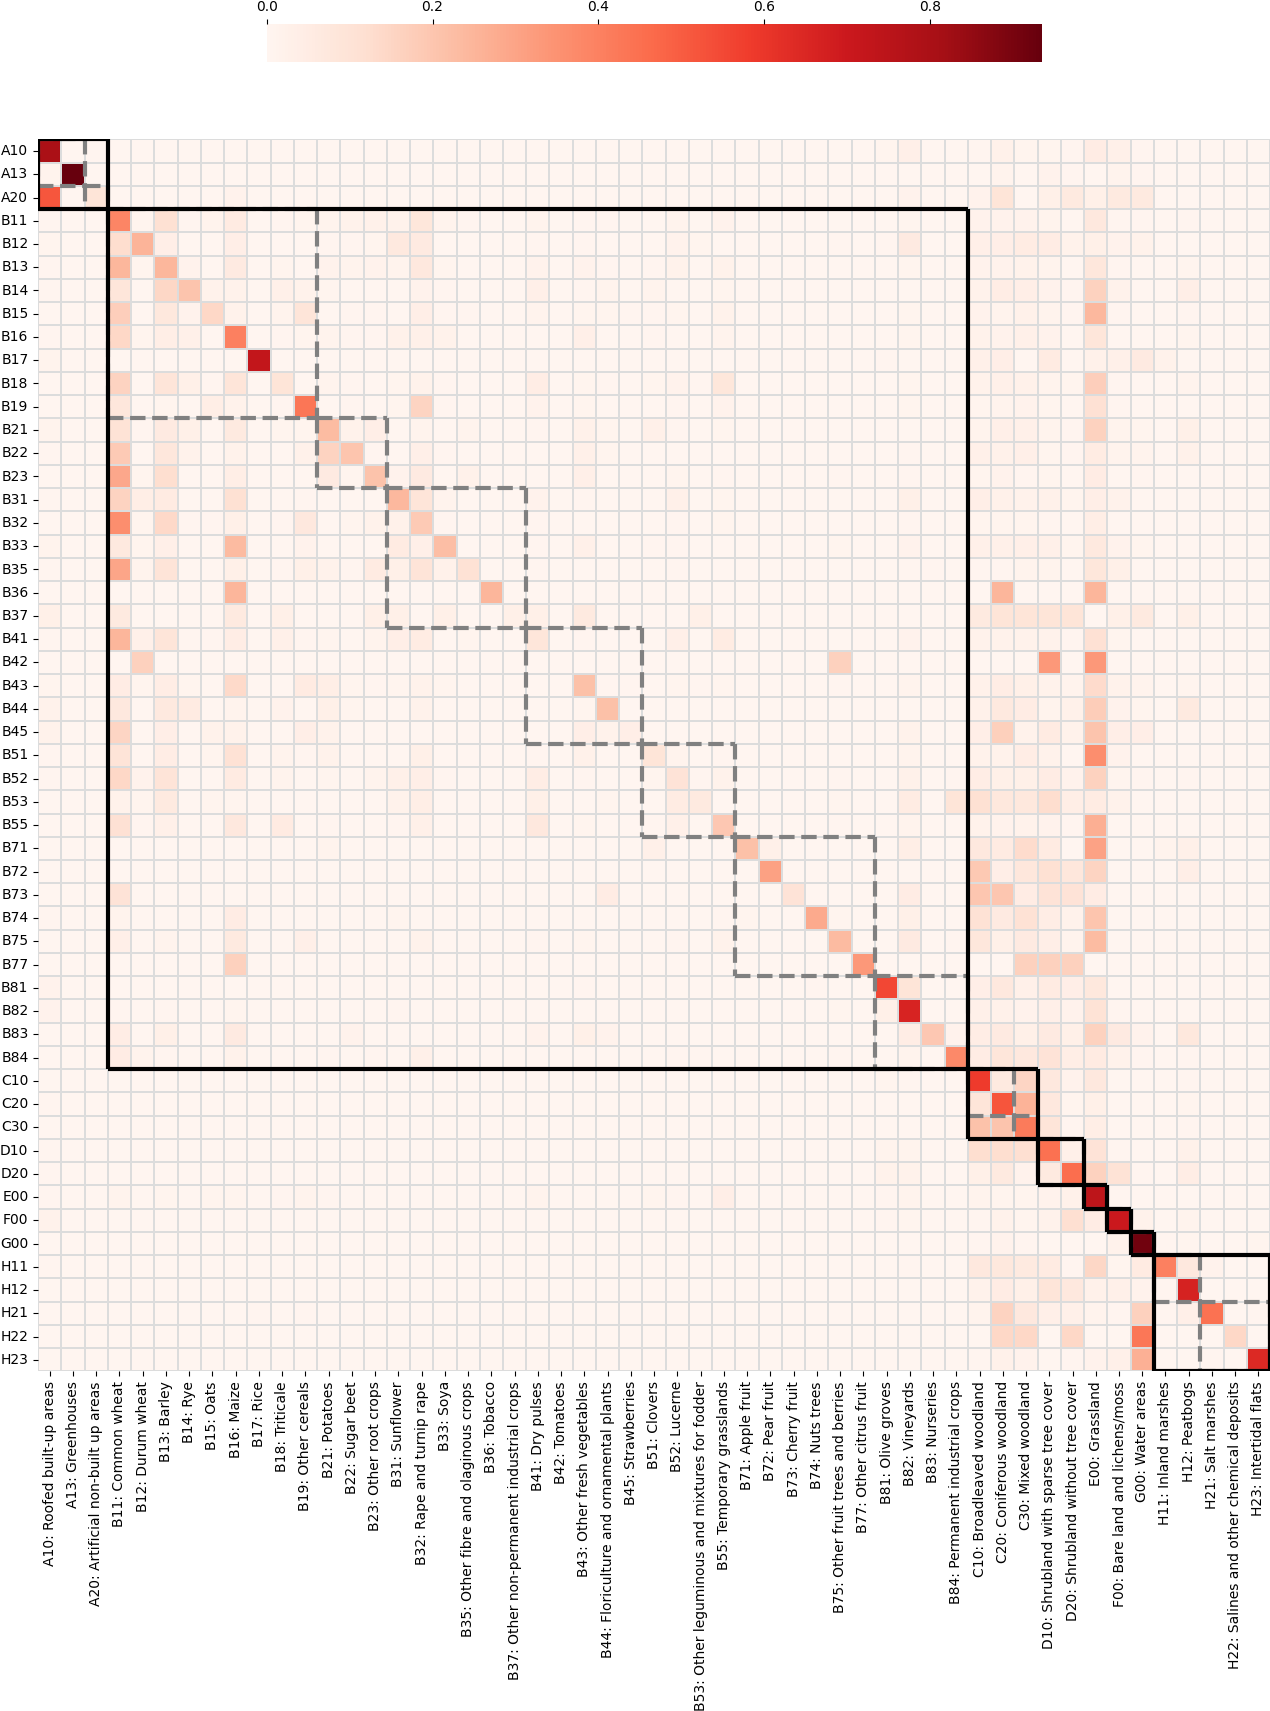
\includegraphics[width=\textwidth]{figs_05/fig_hierarchical_confusion_matrix_calib.png}
        \caption{Confusion matrix of the LUCAS points classified by IMP, normalized based on true class quantities. Red squares mean that the true class (x-axis) was often incorrectly predicted as the predicted class (y-axis)The grey dashed lines indicate which classes belong to the same level 2 class in the hierarchical legend. The black lines indicate level 1 class membership.}
        \label{fig:05_confusion_matrix}
    \end{figure}

    \subsection{Selective Hierarchical Classification}

        Figure~\ref{fig:05_comparison_metrics} shows the highest predicted probability and the margin of victory for maximum probability classification, and the classification iteration for IMP.
        
        \begin{figure}[H]
            \centering
            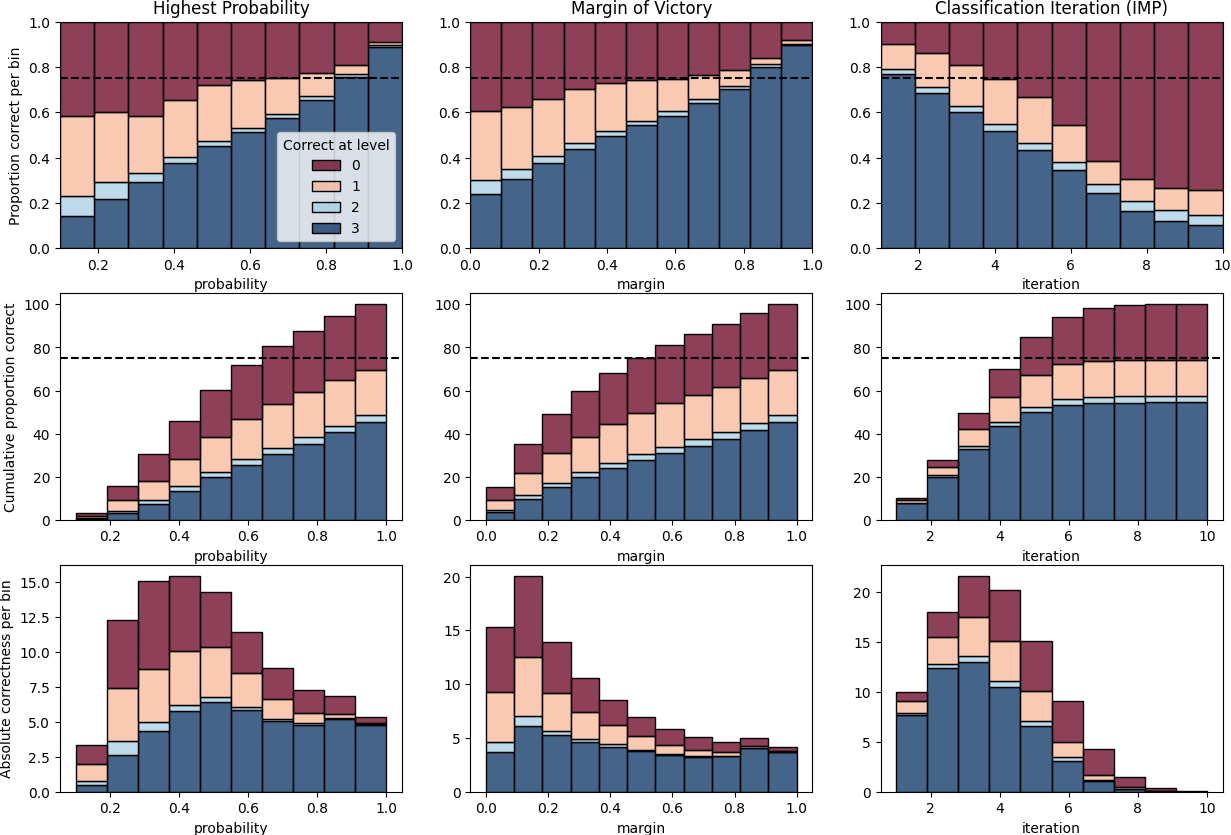
\includegraphics[width=\linewidth]{figs_05/fig_calibration.png}
            \caption{Caption}
            \label{fig:05_comparison_metrics}
        \end{figure}

\section{Discussion}

    \subsection{How to use?}
        selective classification exists; it leaves parts empty. Is it better to have something than nothing?
        how to visualize these maps?
        how to use hierarchical maps in GIS software?
            help focus on areas that need to be studied/sampled better
        how to use their data?
            combine different level predictions into ensembles
        
        

    \subsection{Area estimates and model bias}

        When we applied IMP to classify the calibration points, we used the class proportion of the points themselves as a proxy for the area estimate. The resulting hard-class classification had identical precision and recall for each class. The class proportion of the calibration points can be considered a 'perfect' area estimate because it is a count, and not an estimation by statistics. \citet{witjes2024iterative} noted that precision and recall were more similar in IMP-produced hard class maps than in maximum probability assignment maps, but they were not identical, as in our calibration results in this work. The results from that work were based on area estimates from Eurostat, which have variance and are not perfectly accurate. This suggests that more accurate area estimates might result in proportional maps that have a closer class-wise link between precision and accuracy. If this is correct, IMP can be used to quantify how representative a validation dataset is of its study area.
        
    \subsection{Covariates}
        The current version of the model only uses Landsat bands and no spectral indices. It is likely that its performance will be much higher when this is implemented. 

    \subsection{Legend}
        We lost a lot of detail in our legend because we needed 1) training data, 2) area estimates, and 3) validation points. We had training data for a lot of water \& bare land subclasses. It would be good if Eurostat made area estimates for all LUCAS land cover classes; we could have included them.